\documentclass[hidelinks,12pt]{article}
\usepackage[left=0.25cm,top=1cm,right=0.25cm,bottom=1cm]{geometry}
%\usepackage[landscape]{geometry}
\textwidth = 20cm
\hoffset = -1cm
\usepackage[utf8]{inputenc}
\usepackage[spanish,es-tabla]{babel}
\usepackage[autostyle,spanish=mexican]{csquotes}
\usepackage[tbtags]{amsmath}
\usepackage{nccmath}
\usepackage{amsthm}
\usepackage{amssymb}
\usepackage{mathrsfs}
\usepackage{graphicx}
\usepackage{subfig}
\usepackage{standalone}
\usepackage[outdir=./Imagenes/]{epstopdf}
\usepackage{siunitx}
\usepackage{physics}
\usepackage{color}
\usepackage{float}
\usepackage{hyperref}
\usepackage{multicol}
%\usepackage{milista}
\usepackage{anyfontsize}
\usepackage{anysize}
%\usepackage{enumerate}
\usepackage[shortlabels]{enumitem}
\usepackage{capt-of}
\usepackage{bm}
\usepackage{relsize}
\usepackage{placeins}
\usepackage{empheq}
\usepackage{cancel}
\usepackage{wrapfig}
\usepackage[flushleft]{threeparttable}
\usepackage{makecell}
\usepackage{fancyhdr}
\usepackage{tikz}
\usepackage{bigints}
\usepackage{scalerel}
\usepackage{pgfplots}
\usepackage{pdflscape}
\pgfplotsset{compat=1.16}
\spanishdecimal{.}
\renewcommand{\baselinestretch}{1.5} 
\renewcommand\labelenumii{\theenumi.{\arabic{enumii}})}
\newcommand{\ptilde}[1]{\ensuremath{{#1}^{\prime}}}
\newcommand{\stilde}[1]{\ensuremath{{#1}^{\prime \prime}}}
\newcommand{\ttilde}[1]{\ensuremath{{#1}^{\prime \prime \prime}}}
\newcommand{\ntilde}[2]{\ensuremath{{#1}^{(#2)}}}

\newtheorem{defi}{{\it Definición}}[section]
\newtheorem{teo}{{\it Teorema}}[section]
\newtheorem{ejemplo}{{\it Ejemplo}}[section]
\newtheorem{propiedad}{{\it Propiedad}}[section]
\newtheorem{lema}{{\it Lema}}[section]
\newtheorem{cor}{Corolario}
\newtheorem{ejer}{Ejercicio}[section]

\newlist{milista}{enumerate}{2}
\setlist[milista,1]{label=\arabic*)}
\setlist[milista,2]{label=\arabic{milistai}.\arabic*)}
\newlength{\depthofsumsign}
\setlength{\depthofsumsign}{\depthof{$\sum$}}
\newcommand{\nsum}[1][1.4]{% only for \displaystyle
    \mathop{%
        \raisebox
            {-#1\depthofsumsign+1\depthofsumsign}
            {\scalebox
                {#1}
                {$\displaystyle\sum$}%
            }
    }
}
\def\scaleint#1{\vcenter{\hbox{\scaleto[3ex]{\displaystyle\int}{#1}}}}
\def\bs{\mkern-12mu}



\title{Funciones de Laguerre - 2a. parte \\ \large {Tema 5 - Funciones especiales} \vspace{-3ex}}
\author{M. en C. Gustavo Contreras Mayén}
\date{ }

\pagestyle{fancy}
\fancyhf{}
\rhead{Curso MAF}
\lhead{\leftmark}
\rfoot{\thepage}
\setlength{\headheight}{16pt}%

\def\changemargin#1#2{\list{}{\rightmargin#2\leftmargin#1}\item[]}
\let\endchangemargin=\endlist 


\begin{document}
\maketitle
\fontsize{14}{14}\selectfont
\tableofcontents
\newpage

%Ref. Riley - 18.7 Laguerre functions
\section{Funciones ordinarias de Laguerre.}\label{sec:seccion_01}

La ecuación diferencial de Laguerre es de la forma:
\begin{align}
x \, \sderivada{y} + (1 - x) \, \pderivada{y} + \nu \, y = 0
\label{eq:ecuacion_18_107}
\end{align}
tiene una singularidad regular en $x = 0$ y una singularidad esencial en \break \hfill $x = \infty$. El parámetro $\nu$ es un número real dado, aunque casi siempre toma un valor entero en aplicaciones físicas. La ecuación de Laguerre aparece en la descripción de la función de onda del átomo de hidrógeno, como ya hemos hecho referencia previamente.
\par
Cualquier solución de la ec. (\ref{eq:ecuacion_18_107}) se llama \emph{función de Laguerre}.

\subsection{Solución en series.}

Dado que el punto $x = 0$ es una singularidad regular, podemos encontrar al menos una solución en forma de serie de Frobenius:
\begin{align}
y(x) = \sum_{m=0}^{\infty} a_{m} \, x^{m+r}
\label{eq:ecuacion_18_108}
\end{align}
Sustituyendo esta serie y sus respectivas derivadas en la ec. (\ref*{eq:ecuacion_18_107}), para luego dividir entre $x^{r-1}$, tendremos que:
\begin{align}
\sum_{m=0}^{\infty} \big[ (m + r)(m + r + 1) + (1 - x)(m + r) + \nu \, x \big] \, a_{m} \, x^{m} = 0
\label{eq:ecuacion_18_109}
\end{align}
Haciendo que $x = 0$, de modo que solo quede el término $m = 0$, obtenemos la ecuación de índices $r^{2} = 0$, que trivialmente tiene $r = 0$ como su raíz repetida. Por lo tanto, la ecuación de Laguerre tiene solo una solución de la forma (\ref{eq:ecuacion_18_108}), que de hecho, se reduce a una simple serie de potencias. Sustituyendo $r = 0$ en la ec. (\ref{eq:ecuacion_18_109}) y exigiendo que el coeficiente de $x^{m+1}$ se anule, obtenemos la relación de recurrencia:
\begin{align}
a_{m+1} = \dfrac{m - \nu}{(m + 1)^{2}} \, a_{m}
\end{align}
Como se mencionó anteriormente, en casi todas las aplicaciones físicas, el parámetro $\nu$ toma valores enteros. Por lo tanto, si $\nu = n$, donde $n$ es un número entero no negativo, vemos que:
\begin{align*}
a_{n+1} = a_{n+2} =\ldots = 0
\end{align*}
por lo que nuestra solución a la ecuación de Laguerre es un polinomio de orden $n$. Es una práctica convencional elegir $a_{0} = 1$, por lo que la solución viene dada por:
\begin{align}
L_{n} (x) &= \dfrac{(-1)^{n}}{n!} \left[ x^{n} - \dfrac{n^{2}}{1!} \, x^{n-1} + \dfrac{n^{2}(n - 1)^{2}}{2!} \, x^{n-2} - \ldots + (-1)^{n} \, n! \right] = \label{eq:ecuacion_18_110} \\[0.5em]
&= \sum_{m=0}^{\infty} (-1)^{m} \, \dfrac{n!}{(m!)^{2} \, (n - m)!} \, x^{m} \label{eq:ecuacion_18_111}
\end{align}
donde $L_{n}(x)$ son los llamados \emph{Polinomios ordinarios de Laguerre de orden n}.
\par
Vemos en particular que $L_{n}(0) = 1$. En la siguiente lista presentamos una lista de los primeros polinomios de Laguerre:
\begin{align*}
L_{0} (x) &= 1 \\[0.5em]
L_{1} (x) &= -x + 1 \\[0.5em]
2! \, L_{2} (x) &= x^{2} - 4 \, x + 2 \\[0.5em]
3! \, L_{3} (x) &= -x^{3} + 9 \, x^{2} - 18 \, x + 6 \\[0.5em]
4! \, L_{4} (x) &= x^{4} -16 \, x^{3} + 72 \, x^{2} - 96 \, x + 24 \\[0.5em]
\vdots
\end{align*}
En la figura (\ref{fig:grafica_Laguerre_01}) se puede apreciar una gráfica con los primeros polinomios ordinarios de Laguerre:
\begin{figure}[H]
    \centering
    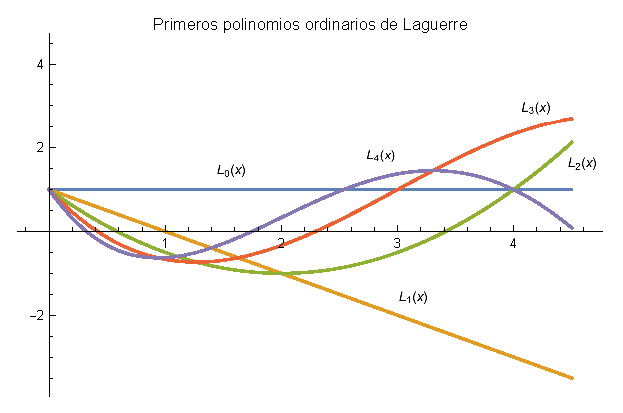
\includegraphics[scale=1.2]{Imagenes/Polinomios_Laguerre_03.eps}
    \caption{Gráfica con los primeros polinomios ordinarios de Legendre $L_{n}(x)$.}
    \label{fig:grafica_Laguerre_01}
\end{figure}

\subsection{Propiedades de los polinomios ordinarios de Laguerre.}
Los polinomios ordinarios de Laguerre y las funciones derivadas de ellos son importantes en el análisis del comportamiento de algunos sistemas físicos en la mecánica cuántica, como lo hemos revisado en los materiales de trabajo previos.
\par
Notarán que el orden en que se revisan las propiedades y características es diferente al que se presentó con los polinomios ordinarios de Legendre, no hay como tal, un orden preciso de revisión, pero si es importante presentar todas las propiedades, en el caso de las relaciones de recurrencia, recuerden que pueden extender las que se presenten en este material de trabajo, para así tener preparada la \enquote{monografía} correspondiente a esta función especial.

\subsubsection{Fórmula de Rodrigues.}

Los polinomios ordinarios de Laguerre puede expresarse en términos de la fórmula de Rodrigues, dada por:
\begin{align}
L_{n} (x) = \dfrac{e^{x}}{n!} \, \dv[n]{x} \left( x^{n} \, e^{-x} \right)
\label{eq:ecuacion_18_112}
\end{align}
la cual puede demostrarse directamente calculando la enésima derivada usando explícitamente el teorema de Leibniz y comparando el resultado con la ec. (\ref{eq:ecuacion_18_111}):
\par
Evaluando la enésima derivada en la ec. (\ref{eq:ecuacion_18_112}) con el teorema de Leibniz, se tiene que:
\begin{align*}
L_{n}(x) &= \dfrac{e^{x}}{n!} \sum_{r=0}^{n} \binom{n}{r} \, \dv[r]{x^{n}}{x} \, \dv[n-r]{e^{-x}}{x} = \\[0.5em]
&= \dfrac{e^{x}}{n!} \sum_{r=0}^{n}  \dfrac{n!}{r! \, (n - r)!} \, \dfrac{n!}{(n - r)!} \, x^{n-r} \, (-1)^{n-r} \, e^{-x} = \\[0.5em]
&= \sum_{r=0}^{n} (-1)^{n-1} \, \dfrac{n!}{r! \, (n - r)! \, (n - r)!} \, x^{n-r}
\end{align*}
al renombrar la suma usando el índice $m = n - r$, se llega a:
\begin{align*}
L_{n}(x) = \sum_{m=0}^{n} (-1)^{m} \, \dfrac{n!}{(m!)^{2} \, (n - m)!} \, x^{m}
\end{align*}
que es la expresión (\ref{eq:ecuacion_18_111}) para el polinomio ordinario de Laguerre de orden $n$.

\subsubsection{Ortogonalidad mutua.}

Un resultado que se revisó en el Tema 3, sabemos que la ecuación de Laguerre es de tipo Sturm Liouville con $p = x \, e^{-x}$, $q = 0$, $\lambda = \nu$ y $\omega = e^{-x}$, y su intervalo natural es entonces $[0, \infty]$.
\par
Dado que los polinomios ordinarios de Laguerre $L_{n} (x)$ son soluciones de la ecuación diferencial y son regulares en los puntos extremos, deben ser mutuamente ortogonales en este intervalo con respecto a la función de peso $\omega = e^{-x}$, es decir:
\begin{align*}
\scaleint{5ex}_{\bs 0}^{\infty} L_{n}(x) \, L_{k} (x) \, e^{-x} \dd{x} = 0 \hspace{0.5cm} \text{si } n \neq k
\end{align*}
Este resultado se puede demostrar usando directamente la fórmula de Rodrigues - ec. (\ref{eq:ecuacion_18_112}). De hecho, la normalización, cuando $k = n$, es más fácil de demostrar usando este método, tendremos entonces que:
\begin{align}
I \equiv \scaleint{5ex}_{\bs 0}^{\infty} L_{n} (x) \, L_{n} (x) \, e^{-x} \dd{x} = 1
\label{eq:ecuacion_18_113}
\end{align}
Usando la fórmula de Rodrigues, podemos escribir:
\begin{align*}
I = \dfrac{1}{n!} \, \scaleint{6ex}_{\bs 0}^{\infty} L_{n}(x) \, \dv[n]{x} \left( x^{n} \, e^{-x} \right) \dd{x} = \dfrac{(-1)^{n}}{n!} \scaleint{6ex}_{\bs 0}^{\infty} \dv[n]{L_{n}}{x} \, x^{n} \, e^{-x} \dd{x}
\end{align*}
en la segunda igualdad se ha integrado por partes $n$ veces y con el hecho de que los términos en los extremos se anulan. Cuando el término $\dv*[n]{L_{n}}{x}$ se evalúa usando la ec. (\ref{eq:ecuacion_18_111}), solo la derivada de $m = n$ términos sobreviven y tienen el valor:
\begin{align*}
\dfrac{(-1)^{n} \, n! \, n!}{(n!)^{2} \, 0!} = (-1)^{n}
\end{align*}
Entonces tenemos que:
\begin{align*}
I = \dfrac{1}{n!} \scaleint{5ex}_{\bs 0}^{\infty} x^{n} \, e^{-x} \dd{x} = 1
\end{align*}
en la segunda igualdad, se ha utilizado la ec. (\ref{eq:ecuacion_18_113}) definiendo la función \break \hfill Gamma.

\subsubsection{Expansión de funciones.}

Las condiciones de normalización y ortogonalidad anteriores nos permiten expandir cualquier función (razonable) en el intervalo $0 \leq x < \infty$ en una serie de la forma:
\begin{align*}
f(x) = \nsum_{n=0}^{\infty} a_{n} \, L_{n} (x)
\end{align*}
en la cual, los coeficientes $a_{n}$ están dado por:
\begin{align*}
a_{n} = \scaleint{5ex}_{\bs 0}^{\infty} f(x) \, L_{n}(x) \, e^{-x} \dd{x}
\end{align*}
Observamos que a veces es conveniente definir las \emph{funciones de Laguerre ortonormales} $\phi_{n} (x) = e^{-x/2} \, L_{n} (x)$, que también pueden usarse para producir una expansión en series de una función en el intervalo $0 \leq x < \infty$.

\subsubsection{Función generatriz.}

La función generatriz para los polinomios ordinarios de Laguerre está dada por:
\begin{align}
G(x, h) = \dfrac{e^{-xh/(1-h)}}{1- h} = \nsum_{n=0}^{\infty} L_{n} (x) \, h^{n}
\label{eq:ecuacion_18_114}
\end{align}

\subsubsection{Relaciones de recurrencia.}\label{sec:subsub_relaciones_recurrencia}

Podemos probar este resultado diferenciando la función generatriz con respecto a $x$ y $h$, respectivamente, para obtener relaciones de recurrencia para los polinomios de Laguerre, que luego pueden combinarse para mostrar que las funciones $L_{n} (x)$ en la ec. (\ref{eq:ecuacion_18_114}) satisfacen efectivamente la fórmula de Laguerre.
\par
Diferenciando la función generatriz (\ref{eq:ecuacion_18_114}) con respecto a $h$, se tiene que:
\begin{align*}
\pdv{G}{h} = \dfrac{(1 - x -h) \, e^{-xh/(1-h)}}{(1- h )^{3}} = \nsum n \, L_{n} \, h^{n-1}
\end{align*}
Por lo que podemos escribir:
\begin{align*}
(1 - x - h) \sum L_{n} \, h^{n} = (1 - h)^{2} \nsum n \, L_{n} \, h^{n-1}
\end{align*}
que al igualar los coeficientes de $h^{n}$ en cada lado de la igualdad, obtenemos:
\begin{align*}
(1 - x) \, L_{n} - L_{n-1} = (n + 1) \, L_{n+1} - 2 \, n \, L_{n} + (n + 1) \, L_{n+1}
\end{align*}
que simplificamos y ordenamos los términos para establecer una relación de recurrencia:
\begin{align}
(n + 1) \, L_{n+1} (x) = (2 \, n + 1 - x) \, L_{n}(x) - n \, L_{n-1} (x)
\label{eq:ecuacion_18_115}
\end{align}
que nos permite encontrar el polinomio ordinario de Laguerre de orden $(n+1)$ a partir de los polinomios de orden $n$ y $n+1$.
\par
Al diferenciar la función generatriz con respecto a $x$, tendremos lo siguiente:
\begin{align*}
\pdv{G}{x} = \dfrac{h \, e^{-xh/(1-h)}}{(1 - h)^{2}} = \sum n \, \pderivada{L}_{n} \, h^{n}
\end{align*}
que nos conduce a:
\begin{align*}
- h \sum L_{n} \, h^{n} =  (1 - h) \, \sum \pderivada{L}_{n} \, h^{n}
\end{align*}
que también al igualar en cada lado los coeficientes de $h^{n}$, llegamos a:
\begin{align}
- L_{n-1} (x) = \pderivada{L}_{n} - \pderivada{L}_{n-1}
\label{eq:ecuacion_18_116}
\end{align}
Haciendo una combinación de los resultados obtenidos en las ecs. (\ref{eq:ecuacion_18_115}) y (\ref{eq:ecuacion_18_116}), es posible obtener una tercera relación de recurrencia:
\begin{align}
x \, \pderivada{L}_{n} (x) = n \, L_{n} (x) - n \, L_{n-1} (x)
\label{eq:ecuacion_18_117}
\end{align}

\section{Funciones asociadas de Laguerre.}

El ecuación diferencial de Laguerre es de la forma:
\begin{align}
x \, \sderivada{y} + (m +  1 - x) \, \pderivada{y} + n \, y = 0
\label{eq:ecuacion_18_118}
\end{align}
tiene una singularidad regular en $x = 0$ y una singularidad esencial en $x = \infty$. Restringimos nuestra atención a la situación en la que los parámetros $n$ y $m$ son números enteros no negativos, como es el caso de casi todos los problemas físicos. La ecuación asociada de Laguerre se presenta con mayor frecuencia en aplicaciones de la mecánica cuántica. Cualquier solución de la ec. (\ref{eq:ecuacion_18_118}) se denomina \emph{función asociada de Laguerre}.
\par
Las soluciones de (18.118) para números enteros no negativos $n$ y $m$ están dadas por los polinomios de asociados de Laguerre:
\begin{align}
L_{n}^{m} (x) = (-1)^{m} \dv[m] L_{n+m} (x) \hspace{1.5cm} m \leq n
\label{eq:ecuacion_18_119}
\end{align}
donde $L_{n}(x)$ son los polinomios ordinarios de Laguerre.
\par
En particular debemos de revisar que $L_{n}^{0} (x) = L_{n}(x)$, ya hemos comentado que $L_{n}(x)$ es un polinomio de orden $n$ por lo que $L_{n}^{m} (x)$ también lo es.
\par
Los primeros polinomios asociados de Laguerre se calculan fácilmente a partir de la ec. (\ref{eq:ecuacion_18_119}):
\begin{align*}
L_{0}^{m} (x) &= 1 \\[0.5em]
L_{1}^{m} (x) &= -x + m + 1 \\[0.5em]
2! \, L_{2}^{m} (x) &= x^{2} - 2 (m + 2) \, x + (m + 1)(m + 2) \\[0.5em]
\vdots
\end{align*}
En la figura (\ref{fig:grafica_Laguerre_02}) se presenta una gráfica con los primeros polinomios asociados de Laguerre.
\begin{figure}[H]
    \centering
    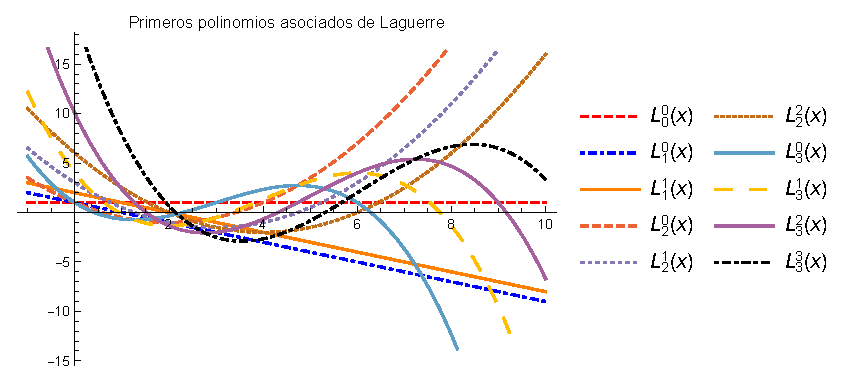
\includegraphics[scale=1]{Imagenes/Polinomios_Laguerre_04.eps}
    \caption{Primeros polinomios asociados de Laguerre.}
    \label{fig:grafica_Laguerre_02}
\end{figure}
De hecho, en el caso general, se puede demostrar directamente, a partir de la definición (\ref{eq:ecuacion_18_119}) y la ec. (\ref{eq:ecuacion_18_111}) para los polinomios ordinarios de Laguerre, que:
\begin{align}
L_{n}^{m} (x) = \sum_{k=0}^{n} (-1)^{k} \, \dfrac{(n + m)!}{k! \, (n - k)! \, (k + m)!} \, x^{k}
\label{eq:ecuacion_18_120}
\end{align}

\subsection{Propiedades de los polinomios asociados de Laguerre}

Las propiedades de los polinomios asociados de Laguerre se derivan directamente de las de los polinomios ordinarios de Laguerre a través de la definición ec. (\ref{eq:ecuacion_18_119}). Por lo tanto, aquí sólo describiremos brevemente los resultados más útiles.

\subsubsection{Fórmula de Rodrigues.}

La fórmula de Rodrigues de los polinomios asociados de Laguerre está dada por la expresión:
\begin{align}
L_{n}^{m} (x) = \dfrac{e^{x} \, x^{-m}}{n!} \, \dv[n]{x} \left( x^{n+m} \, e^{-x} \right)
\label{eq:ecuacion_18_121}
\end{align}
Que se puede demostrar al evaluar la enésima derivada usando el teorema de Leibniz.

\subsubsection{Ortogonalidad mutua.}

Del Tema 3 del curso sabemos que la ecuación diferencial asociada de Laguerre es de tipo Sturm Liouville con $p = x^{m+1} \, e^{-x}$, $q = 0$, $\lambda = n$ y $\omega = x^{m} \, e^{-x}$, y su intervalo natural es entonces $[0, \infty]$.
\par
Dado que los polinomios asociados de Laguerre $L_{m}^{n} (x)$ son soluciones de la ecuación y son regulares en los puntos extremos, aquellos con el mismo $m$ pero valores diferentes del valor propio $\lambda = n$ deben ser mutuamente ortogonales en este intervalo con respecto a la función de peso $\omega = x^{m} \, e^{-x}$, es decir:
\begin{align*}
\scaleint{5ex}_{\bs 0}^{\infty} L_{n}^{m} (x) \, L_{k}^{m} (x) \, x^{m} \, e^{-x} \dd{x} = 0 \hspace{1.5cm} \mbox{si } n \neq k
\end{align*}
Este resultado también se puede demostrar utilizando la fórmula de Rodrigues (\ref{eq:ecuacion_18_121}), al igual que la condición de normalización cuando $k = n$:
\begin{align}
I \equiv \scaleint{5ex}_{\bs 0}^{\infty} L_{n}^{m} (x) \, L_{n}^{m} (x) \, x^{m} \, e^{-x} \dd{x} =\dfrac{(n + m)!}{n!}
\label{eq:ecuacion_18_122}
\end{align}
Usando la fórmula de Rodrigues (\ref{eq:ecuacion_18_121}), podemos escribir:
\begin{align*}
I = \dfrac{1}{n!} \scaleint{6ex}_{\bs 0}^{\infty} L_{n}^{m} \, \dv[n]{x} \left( x^{n+m} \, e^{-x} \right) \dd{x} = \dfrac{(-1)^{n}}{n!} \scaleint{6ex}_{\bs 0}^{\infty} \dv[n]{L_{n}^{m}}{x} \, x^{n+m} \, e^{-x} \dd{x}
\end{align*}
en la segunda igualdad se ha integrado por partes $n$ veces y se ha utilizado el hecho de que los términos en los extremos se anulan. De la ec. (\ref{eq:ecuacion_18_120}) tenemos que 
\begin{align*}
I = \dfrac{1}{n!} \scaleint{5ex}_{\bs 0}^{\infty} x^{n+m} \, e^{-x} \dd{x} = \dfrac{(n + m)!}{n!}
\end{align*}
en la segunda igualdad, se ha ocupado la definición de la función Gamma.

\subsubsection{Expansión de funciones.}

Dada las condiciones de ortogonalidad y normalización, es posible expandir cualquier función (razonable) en el intervalo $0 \leq x < \infty$ en una serie de la forma:
\begin{align*}
f(x) = \nsum_{n=0}^{\infty} a_{n} \, L_{n}^{m} (x)
\end{align*}
en la cual, los coeficientes $a_{n}$ están dado por la expresión:
\begin{align*}
a_{n} = \dfrac{n!}{(n + m)!} \scaleint{5ex}_{\bs 0}^{\infty} f(x) \, L_{n}^{m}(x) \, x^{m} \, e^{-x} \dd{x}
\end{align*}
Es conveniente conocer que en ocasiones se definen las \emph{funciones ortogonales asociadas de Laguerre}:
\begin{align*}
\phi_{n}^{m} (x) = x^{m/2} \, e^{-x/2} \, L_{n}^{m} (x)
\end{align*}
que también se puede utilizar para producir una expansión en series de una función en el intervalo $0 \leq x < \infty$.

\subsubsection{Función generatriz.}

La función generatriz de los polinomios asociados de Laguerre están dados por:
\begin{align}
G(x, h) = \dfrac{\exp\big[(-x \, h)/(1 - h)\big]}{(1 - h)^{m+1}} = \nsum_{n=0}^{\infty} L_{n}^{m} (x) \, h^{n}
\label{eq:ecuacion_18_123}
\end{align}
Esta expresión se obtiene al diferenciar $m$ veces con respecto a $x$ la función generatriz (\ref{eq:ecuacion_18_114}) de los polinomios ordinarios de Laguerre y ocupando la ec. (\ref{eq:ecuacion_18_119}).
\par
Como ejemplo del uso de la función generatriz veamos su manejo para obtener una expresión de $L_{n}^{m}(0)$:
\par
Tenemos entonces que:
\begin{align*}
&\nsum_{n=0}^{\infty} L_{n}^{m} (0) \, h^{n} = \dfrac{1}{(1 - h)^{m+1}} = \\[0.5em]
&= 1 + (m + 1) \, h + \dfrac{(m + 1)(m + 2)}{2!} \, h^{2} + \ldots + \\[0.5em]
&+ \dfrac{(m + 1)(m + 2) \ldots (m + n)}{n!} \, h^{n} + \ldots  
\end{align*}
en la segunda igualdad, se ha expandido el lado derecho usando el teorema del binomio. Al igualar los coeficientes de $h^{n}$, se obtiene:
\begin{align*}
L_{n}^{m} (0) = \dfrac{(n + m)!}{n! \, m!}
\end{align*}

\subsubsection{Relaciones de recurrencia.}

Las distintas relaciones de recurrencia por los polinomios asociados de Laguerre se obtienen diferenciando la función generadora (\ref{eq:ecuacion_18_123}) con respecto a uno o ambos de $x$ y $h$, o diferenciando con respecto a $x$ las relaciones de recurrencia de los polinomios ordinarios de Laguerre, discutidos en la subsección (\ref{sec:subsub_relaciones_recurrencia}). De las relaciones de recurrencia de los polinomios asociados de Laguerre, se presentan a continuación las más útiles:
\begin{align}
(n + 1) \, L_{n+1}^{m} (x) &= (2 \, n + m + 1 - x) \, L_{n}^{m} (x) - (n + m) \, L_{n-1}^{m} (x) \label{eq:ecuacion_18_124} \\[0.5em]
x \, \pderivada{(L_{n}^{m})} (x) &= n \, L_{n}^{m} (x) - (n + m) \, L_{n-1}^{m} (x) \label{eq:ecuacion_18_125} \\[0.5em]
\pderivada{L_{n}^{m}} &= - L_{n-1}^{m+1} (x) \label{eq:ecuacion_18_125a} \\[0.5em]
L_{n}^{m} (x) &= L_{n}^{m+1} (x) - L_{n-1}^{m+1} (x) \label{eq:ecuacion_18_125b} \\[0.5em]
n \, L_{n}^{m} (x) &= (n + m) \, L_{n-1}^{m} (x) - x \, L_{n-1}^{m+1} (x) \label{eq:ecuacion_18_125c}
\end{align}

\newpage
\section{Ejercicios a cuenta.}

%Ref. Andrews (1998) Special Functions Chap. 5 Problem 11
\noindent
\textbf{Ejercicio a cuenta (45).} Demuestra la siguiente fórmula integral con los polinomios ordinarios de Laguerre:
\begin{align*}
\scaleint{6ex}_{\bs 0}^{\infty} e^{-x} \, x^{k} \, L_{n}(x) \dd{x} = \begin{cases}
0 & k < n \\
(-1)^{n} \, n! & k = n
\end{cases}
\end{align*}


%Ref. Arfken (2006)
\noindent
\textbf{Ejercicio a cuenta (46).} Demuestra que la expansión de la función \break \hfill $f(x) =x^{r}$ en una serie de polinomios asociados de Laguerre $L_{n}^{k}(x)$, con $k$ fijo y $n$ variando de $0$ a $r$ (o variando $r$ a $\infty$, si $r$ es un no entero) es:
\begin{align*}
x^{r} = (r + k)! \, r! \nsum_{n=0}^{r} \dfrac{(-1)^{n} \, L_{n}^{k}(x)}{(n + k)! \, (r - n)!} \hspace{1.5cm} 0 \leq x < \infty
\end{align*}
Nota: Considera que la fórmula de Rodrigues de los $L_{n}^{k}(x)$ puede ser de utilidad.

\end{document}